\documentclass[aspectratio=169]{beamer}
\usetheme{simple}
\usepackage[english]{babel}
\usepackage[utf8]{inputenc}
\usepackage{lmodern} 
\usefonttheme[onlymath]{serif}
\usepackage[scale=2]{ccicons} 

\usepackage{graphicx,hyperref,url,pgfplots}
\usepackage{media9}
\usepackage{amsmath} 
\usepackage{array,booktabs}
\usepackage{pdfpages}
\pgfplotsset{compat=1.13}  
\pgfplotsset{width=7cm}


\setbeamercovered{invisible} 
\newcommand{\pausar}{\pause}
\newcommand{\df}[1]{\,\mathrm{d}#1}
\newcommand{\parcial}[3]{\dfrac{\partial^{#1}#2}{\partial #3^{#1}}}

\usepackage{tikz}
\usepackage{xcolor}
\usetikzlibrary{scopes}
\usepackage{verbatim}
\usetikzlibrary{patterns}
\usepackage{algorithm}
\usepackage{algpseudocode}

\usepackage{listings}
	\definecolor{codegreen}{rgb}{0,0.6,0}
	\definecolor{codegray}{rgb}{0.5,0.5,0.5}
	\definecolor{codepurple}{rgb}{0.58,0,0.82}
	\definecolor{backcolour}{rgb}{0.92,0.92,0.92}
	\lstset{language=Python, 
	backgroundcolor=\color{backcolour},   
	commentstyle=\color{codegreen},
	keywordstyle=\color{magenta},
	numberstyle=\tiny\color{codegray},
	stringstyle=\color{codepurple},
	basicstyle=\fontsize{8}{11}\ttfamily,
	frame=lines,
%	numbers=left,
	tabsize=2,
	morekeywords={models, lambda, forms}}


\title{Mobile Robots}
\subtitle{Extended Kalman Filter Algorithm}
\date{\today}
\author[Jeferson José de Lima]{
\textbf{Professor}: Jeferson José de Lima}
\institute{Academic Department of Informatics (DAINF) \\ Federal University of Technology - Paraná (UTFPR) at Pato Branco, PR, Brazil}

\begin{document}

\maketitle

\begin{frame}{Useful Information}
	\begin{block}{Material disponível em:}
		\href{Robótica Móvel - Wiki}{https://gitlab.com/cursoseaulas/robotica-movel/-/wikis/home}
	\end{block}
\end{frame}

\begin{frame}[c]{Extended Kalman Filter}
    \framesubtitle{Introdução}
    \begin{itemize}
        \item \textcolor{red}{Sistema do Mundo Real não são lineares};
        \item O filtro de Kalman foi desenvolvido para sistemas lineares, e normalmente assume-se que todas as perturbações e ruídos podem ser descritos com uma distribuição gaussiana de média zero;
        \item \textcolor{blue}{Se qualquer uma das transições de estado ou equações de saída do sistema for uma função não linear}, o filtro de Kalman convencional pode não mais produzir uma estimativa de estado ideal. Para contornar o problema das não linearidades, um \textcolor{blue}{Extended Kalman Filter (EKF) foi desenvolvido}, onde as não linearidades do sistema são aproximadas com modelos lineares locais;
        \item \textbf{Portanto, o algoritmo EKF é comumente usado na prática};
    \end{itemize}

\end{frame}


\begin{frame}[c]{Extended Kalman Filter}
    \framesubtitle{Introdução}
    \begin{itemize}
        \item Um exemplo clássico de sistemas considerado puramente linear é o do resistor,


    \begin{figure}
        \centering
        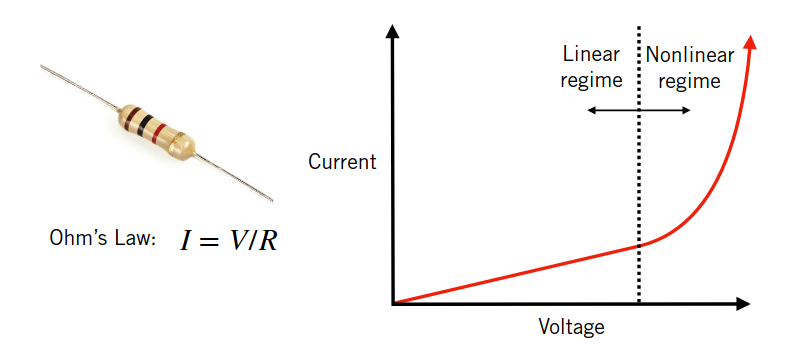
\includegraphics[width=0.7\textwidth]{./images/resistor_curve.png}
        \caption{Curva experimental de corrente vs tensão Resistor}
    \end{figure}

        \item Neste caso, o resistor tem um compartamento linear até determinada faixa de operação.
    \end{itemize}
\end{frame}


\begin{frame}[t]{Extended Kalman Filter}
    \framesubtitle{Sistemas Não Lineares}

    \begin{itemize}
        \item Problemas de Robótica Móvel mais realistas envolvem equação não lineares.
        \item Um sistema não linear pode ser escrito de uma forma geral:
        
        \begin{equation}
            \begin{split}
            x_t = & g(u_t, x_{t-1})\\
            z_t = & h(x_t)
            \end{split}
        \end{equation}
    
    onde $g(u_t, x_{t-1})$ e $h(x_t)$ são funções não lineares que representam, consecutivamente, 
    o modelo do sistema e o modelo dos sensores.

    \end{itemize}

    \begin{block}{Então como resolver esse problema?}
        \centering
        \Large{\textcolor{red}{Linearização do Sistema}}
    \end{block}

\end{frame}

\begin{frame}[c]{Extended Kalman Filter}
    \framesubtitle{Linearização de sistemas}
    \begin{itemize}
        \item Podemos achar função linear do sistema no ponto $\color{red}{a}$ através da Expansão da Série de Taylor. Um exemplo interativo: \href{https://www.desmos.com/calculator/oiexhzavjp}{link}.

    \begin{figure}
        \centering
        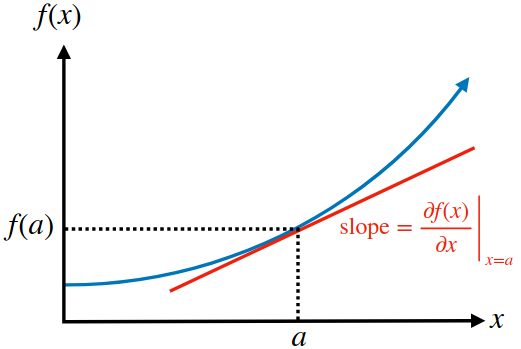
\includegraphics[width=0.4\textwidth]{./images/taylor.png}
    \end{figure}

        \begin{equation}
            f(x) = \color{red}{f(a) + \left. \frac{\partial f(x)}{\partial x} \right\vert_{x=a}(x-a)} + 
            \color{gray}{\frac{1}{2!}\left. \frac{\partial^2 f(x)}{\partial^2 x} \right\vert_{x=a}(x-a)^2 + \cdots}
        \end{equation}

        \item Para o EKF, \textcolor{red}{apenas a aproximação de primeira ordem é utilizada}.
    \end{itemize}

\end{frame}




\begin{frame}[c]{Extended Kalman Filter}
    \framesubtitle{Linearização de sistemas}
        \begin{block}{Prediction}
            \begin{equation*}
                \begin{split}
                    g(u_t, x_{t-1} \approx & g(u_t, \mu_{t-1}) + \frac{\partial g(u_t, \mu_{t-1}) }{\partial x_{t-1}}(x_{t-1}-\mu_{t-1}) \\
                    g(u_t, x_{t-1} \approx & g(u_t, \mu_{t-1}) + \color{red}{G_t}\color{gray}{(x_{t-1}-\mu_{t-1})}
                \end{split}
            \end{equation*}
            onde $\color{red}G_t$ é calculado pela Matriz Jacobiana.
        \end{block}


        \begin{block}{Measurement Update}
            \begin{equation*}
                \begin{split}
                    h(x_t) \approx & h(\overline{\mu}_t) + \frac{\partial h(\overline{\mu}_t) }{\partial x_{t}}(x_{t}-\overline{\mu}_{t}) \\
                    h(x_t) \approx & h(\overline{\mu}_t) + \color{blue}{H_t}\color{gray}{(x_{t}-\overline{\mu}_{t})}
                \end{split}
            \end{equation*}
            onde $\color{blue}H_t$ é calculado pela Matriz Jacobiana.
        \end{block}

\end{frame}

\begin{frame}[c]{Extended Kalman Filter}
    \framesubtitle{Linearização de sistemas}
       A matrix Jacobiana é data por:
        \begin{equation*}
        \mathbb{J}
        =
        \frac{d \mathbf{f}}{d \mathbf{x}}
        =
        \left[ \frac{\partial \mathbf{f}}{\partial q_1}
            \cdots \frac{\partial \mathbf{f}}{\partial x_n} \right]
        =
        \begin{bmatrix}
            \frac{\partial f_1}{\partial x_1} & \cdots &
            \frac{\partial f_1}{\partial x_n}                   \\
            \vdots                            & \ddots & \vdots \\
            \frac{\partial f_m}{\partial x_1} & \cdots &
            \frac{\partial f_m}{\partial x_n}
        \end{bmatrix}
    \end{equation*}
    
    \begin{block}{Exemplo}
        dado um sistema representado por $\mathbf{F(x)}$, calcule a
    matriz jacobina do sistema:
    
    \begin{equation*}
        \mathbf{F(x)}
        =
        \begin{bmatrix}
            f_1 \\
            f_2
        \end{bmatrix}
        =
        \begin{bmatrix}
            x_1 + x_2 \\
            x_1^2
        \end{bmatrix}
    \end{equation*}
    
    logo:

    \begin{equation*}
        \frac{d \mathbf{f(x)}}{d \mathbf{x}}
        =
        \begin{bmatrix}
            \frac{\partial f_1}{\partial x_1} &
            \frac{\partial f_1}{\partial x_2} \\
            \frac{\partial f_2}{\partial x_1} &
            \frac{\partial f_2}{\partial x_2}
        \end{bmatrix}
        =
        \begin{bmatrix}
            1 & 1 \\
            2x_1 & 0
        \end{bmatrix}
    \end{equation*}
\end{block}


\end{frame}


\begin{frame}[c]{Extended Kalman Filter}
    \framesubtitle{Algoritmo}
    \begin{algorithm}[H]
        \caption{Extended-Kalman-Filter}
        \begin{algorithmic}[1]
        \Procedure{Prediction}{$\mu_{t-1}, {\textstyle\sum}_{t-1}, u_t$}
            \State $\overline{\mu}_t = g(u_t, \mu_{t-1})$
            \State $ \overline{\textstyle\sum}_t = G_t {\textstyle\sum}_{t-1} G_t^T+ Q_t$ 
            \State \textbf{Return} $\left(\overline{\mu}_t, \overline{\textstyle\sum}_t\right)$
        \EndProcedure
        \Procedure{Update}{$\overline{\mu}_{t}, \overline{\textstyle\sum}_{t}, z_t$}
            \State $K_t = \overline{\textstyle\sum}_tH_t^T(H_t\overline{\textstyle\sum}_tH_t^T+R_t)^{-1}$
            \State $\mu_t  = \overline{\mu}_t + K_t(z_t -h(\overline\mu_t))$
            \State{$\textstyle\sum_t = (I-K_t H_t)\overline{\textstyle\sum}_t$}
            \State \textbf{Return} $\left(\mu_t, \textstyle\sum_t\right)$
        \EndProcedure
        \end{algorithmic}
    \end{algorithm}
\end{frame}


\begin{frame}[c]{Extended Kalman Filter}
    \framesubtitle{Exercício - Deslocamento Carro - Extended Kalman Filter}    \begin{columns}
        \begin{column}[c]{0.4\textwidth}
            \begin{figure}
                \centering
                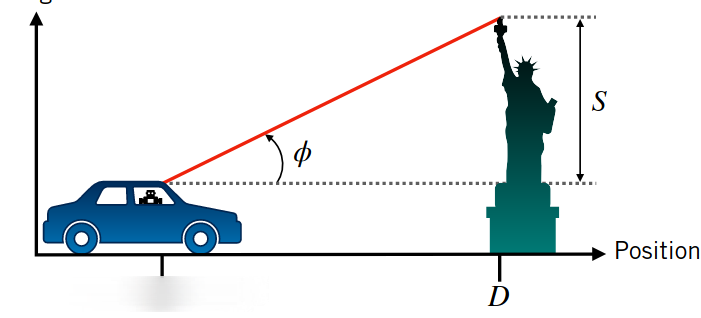
\includegraphics[width=1\textwidth]{./images/kalman_car2.png}
                \caption{Exemplo Deslocamento Carro}
            \end{figure}
        
        Tempo contínuo
        \begin{equation*}
           \left\{
            \begin{matrix}
                s = & s_0 + vt \\
                v = & v_0 + at
            \end{matrix}, 
            \quad
            \mathbf{x} = 
            \begin{bmatrix}
                x \\
                \dot{x}
            \end{bmatrix},
            \right.
        \end{equation*}
        
        \begin{equation*}
            \text{e, }\mathbf{u}=a
        \end{equation*}

        \end{column}
        \begin{column}[c]{0.6\textwidth}
            
            \textbf{Eq. Movimento - Tempo Discreto}:

            \begin{equation*}
                \mathbf{x}_t = 
                \begin{bmatrix}
                        1 & \Delta t \\
                        0 & 1
                \end{bmatrix}
                \mathbf{x}_{t-1} +
                \begin{bmatrix}
                        0 \\
                        \Delta t
                \end{bmatrix}
                \mathbf{u}_{t-1} +
                \mathbf{w}_{t-1}
            \end{equation*}

            \textbf{Eq. Sensor - Tempo Discreto}:

            \begin{equation*}
                \mathbf{z}_t = \phi_t  = 
                \tan^{-1}\left(\frac{S}{D-x_t} \right) +
                v_{t}
            \end{equation*}            

            \textbf{Ruído}:

            $\mathbf{w}_t \sim \mathcal{N} 
                \left(
                    \begin{bmatrix}
                    0 \\ 0    
                    \end{bmatrix},
                    \begin{bmatrix}
                    0.1 & 0 \\
                    0   & 0.1
                \end{bmatrix}
                \right)$ e :
            
            $ v_t \sim \mathcal{N} (0,0.05)$

        \end{column}
    \end{columns}
\end{frame}



\begin{frame}[c]{Extended Kalman Filter}
    \framesubtitle{Exercício - Deslocamento Carro - Extended Kalman Filter}
    
    \begin{itemize}
        \item 1) Dado o sistema que descreve o deslocamento do carro acima,
        calcule o primeiro passo do algoritmo Extended Kalman Filter.
    \end{itemize}

    \begin{columns}
        \begin{column}[c]{0.4\textwidth}
            \begin{figure}
                \centering
                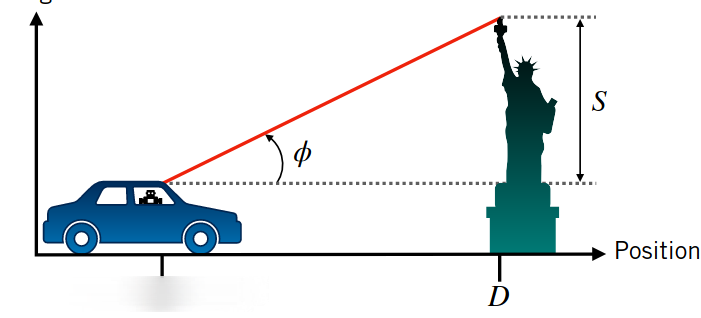
\includegraphics[width=1\textwidth]{./images/kalman_car2.png}
                \caption{Exemplo Deslocamento Carro}
            \end{figure}
            
        \end{column}
        \begin{column}[c]{0.6\textwidth}
            
            \textbf{Condições Iniciais}:

            \begin{equation*}
                \mu_0 \sim \mathcal{N} \left( 
                    \begin{bmatrix}
                        0 \\ 5
                    \end{bmatrix}, 
                    \begin{bmatrix}
                        0.01 & 0 \\
                        0 & 1
                    \end{bmatrix} \right)
            \end{equation*}

            $\Delta t = 0.5s$

            $u_0 = -2m/s^2$

           $z_1 = \frac{\pi}{6} rad$ 

           $D = 40m$

           $S = 20m$

        \end{column}
    \end{columns}
\end{frame}



\begin{frame}[t]{Referências}

    \begin{itemize}
        \item Sebastian Thrun, Wolfram Burgard, Dieter Fox. Probabilistic Robotics (Intelligent Robotics and Autonomous Agents series). The MIT Press, 2005.
        \item Roland Siegwart, Illah Reza Nourbakhsh, Davide Scaramuzza. Introduction to Autonomous Mobile Robots (Intelligent Robotics and Autonomous Agents series), 2nd ed. The MIT Press, 2011.
    \end{itemize}

\end{frame}
\end{document}



% % https://classroom.udacity.com/courses/ud810/